\documentclass[sigconf]{acmart}

\usepackage{booktabs} % For formal tables
\usepackage{algorithm}
\usepackage{algorithmic}
\usepackage{subfigure}
\usepackage{url}
\usepackage{amsmath}

% Copyright
% \setcopyright{none}
%\setcopyright{acmcopyright}
%\setcopyright{acmlicensed}
\setcopyright{rightsretained}
%\setcopyright{usgov}
%\setcopyright{usgovmixed}
%\setcopyright{cagov}
%\setcopyright{cagovmixed}


% DOI
\acmDOI{}

% ISBN
% \acmISBN{123-4567-24-567/08/06}

%Conference
\acmConference[ISMSI'18]{3rd International Conference on Intelligent Systems, Metaheuristics \& Swarm Intelligence}{March 23-24 2019}{Male, Moldives}
\acmYear{2019}
% \copyrightyear{}


% \acmArticle{}
% \acmPrice{}

% These commands are optional
%\acmBooktitle{Transactions of the ACM Woodstock conference}
% \editor{}
% \editor{}
% \editor{}

\begin{document}
\title{The Bat Algorithm with Dynamic Niche Radius for Multimodal Optimization}
% \titlenote{Produces the permission block, and
  % copyright information}
% \subtitle{Extended Abstract}
% \subtitlenote{The full version of the author's guide is available as
  % \texttt{acmart.pdf} document}


\author{Takuya Iwase}
% \authornote{Dr.~Trovato insisted his name be first.}
% \orcid{1234-5678-9012}
\affiliation{%
  \institution{The University of Electro-Communications}
  % \streetaddress{P.O. Box 1212}
  \city{Tokyo}
  \country{Japan}
  % \postcode{43017-6221}
}
\email{tanu_iwa@cas.lab.uec.ac.jp}

\author{Ryo Takano}
% \authornote{The secretary disavows any knowledge of this author's actions.}
\affiliation{%
  \institution{The University of Electro-Communications}
  % \streetaddress{P.O. Box 1212}
  \city{Tokyo}
  \country{Japan}
  % \postcode{43017-6221}
}
\email{takano@cas.lab.uec.ac.jp}

\author{Fumito Uwano}
% \authornote{This author is the
  % one who did all the really hard work.}
\affiliation{%
  \institution{The University of Electro-Communications}
  % \streetaddress{1 Th{\o}rv{\"a}ld Circle}
  \city{Tokyo}
  \country{Japan}}
\email{uwano@cas.lab.uec.ac.jp}

\author{Hiroyuki Sato}
% \authornote{The secretary disavows any knowledge of this author's actions.}
\affiliation{%
  \institution{The University of Electro-Communications}
  % \streetaddress{P.O. Box 1212}
  \city{Tokyo}
  \country{Japan}
  % \postcode{43017-6221}
}
\email{h.sato@uec.ac.jp}

\author{Keiki Takadama}
% \authornote{This author is the
  % one who did all the really hard work.}
\affiliation{%
  \institution{The University of Electro-Communications}
  % \streetaddress{1 Th{\o}rv{\"a}ld Circle}
  \city{Tokyo}
  \country{Japan}}
\email{keiki@inf.uec.ac.jp}

% \author{Valerie B\'eranger}
% \affiliation{%
%   \institution{Inria Paris-Rocquencourt}
%   \city{Rocquencourt}
%   \country{France}
% }
% \author{Aparna Patel}
% \affiliation{%
%  \institution{Rajiv Gandhi University}
%  \streetaddress{Rono-Hills}
%  \city{Doimukh}
%  \state{Arunachal Pradesh}
%  \country{India}}
% \author{Huifen Chan}
% \affiliation{%
%   \institution{Tsinghua University}
%   \streetaddress{30 Shuangqing Rd}
%   \city{Haidian Qu}
%   \state{Beijing Shi}
%   \country{China}
% }

% \author{Charles Palmer}
% \affiliation{%
%   \institution{Palmer Research Laboratories}
%   \streetaddress{8600 Datapoint Drive}
%   \city{San Antonio}
%   \state{Texas}
%   \postcode{78229}}
% \email{cpalmer@prl.com}

% \author{John Smith}
% \affiliation{\institution{The Th{\o}rv{\"a}ld Group}}
% \email{jsmith@affiliation.org}

% \author{Julius P.~Kumquat}
% \affiliation{\institution{The Kumquat Consortium}}
% \email{jpkumquat@consortium.net}

% The default list of authors is too long for headers.
% \renewcommand{\shortauthors}{B. Trovato et al.}


\begin{abstract}
In this paper, we proposed Bat Algorithm extending with Dynamic Niche Radius (DNRBA) which enables solutions to locate multiple local and global optima for solving multimodal optimization problems. This proposed algorithm is designed Bat Algorithm (BA) dealing with the exploration and the exploitation search with Niche Radius which is calculated by the fitness landscape and the number of local and global optima to avoid converging solutions at the same optimum. Although the Niche Radius is an effective niching method for locating solutions at the peaks in the fitness landscape, it is not applicable for uneven multimodal functions and easily fails to keep multiple optima. To overcome this problem, we introduce a dynamic niche sharing scheme which is able to adjust the distance of the niche radius in the search process dynamically for the BA. In the experiment, we employ several multimodal functions and compare DNRBA with the conventional BA to evaluate the performance of DNRBA.
\end{abstract}

%
% The code below should be generated by the tool at
% http://dl.acm.org/ccs.cfm
% Please copy and paste the code instead of the example below.
%
\begin{CCSXML}
<ccs2012>
 <concept>
  <concept_id>10010520.10010553.10010562</concept_id>
  <concept_desc>Mathematics of computing~Bio-inspired optimization</concept_desc>
  <concept_significance>500</concept_significance>
 </concept>
%  <concept>
%   <concept_id>10010520.10010575.10010755</concept_id>
%   <concept_desc>Computer systems organization~Redundancy</concept_desc>
%   <concept_significance>300</concept_significance>
%  </concept>
%  <concept>
%   <concept_id>10010520.10010553.10010554</concept_id>
%   <concept_desc>Computer systems organization~Robotics</concept_desc>
%   <concept_significance>100</concept_significance>
%  </concept>
%  <concept>
%   <concept_id>10003033.10003083.10003095</concept_id>
%   <concept_desc>Networks~Network reliability</concept_desc>
%   <concept_significance>100</concept_significance>
%  </concept>
% </ccs2012>
\end{CCSXML}

\ccsdesc[500]{Mathematics of computing~Bio-inspired optimization}
% \ccsdesc[300]{Computer systems organization~Redundancy}
% \ccsdesc{Computer systems organization~Robotics}
% \ccsdesc[100]{Networks~Network reliability}


\keywords{Bat Algorithm, Multimodal optimization, Swarm Intelligence, Niching method}


\maketitle


\section{Introduction}

In the past couple of decades, metaheuristic algorithms became major method for optimization problem. Generally, they are based on biological evolution in nature-inspired system. 
% These various methods are adaptable for a specific situation using non-linear objective functions.
 Particle Swarm Optimization (PSO) which is one of metaheuristic algorithms, modeled fish swarm if a fish find a global optimum, the other fishes converge to the fish \cite{PSO01}. Meanwhile, there is another algorithm called Firefly Algorithm (FA), which is particularly well to local search with flashing light of fireflies \cite{FA01}. In two fireflies, a brighter firefly attracted the other one. Although these algorithms are widely used for optimization problem, the performance of search considerably depends on the scale and contour of multimodal functions. To adapt any optimization problem, we have to consider the balance of performance which unites global search and local search. Bat algorithm (BA) is one of bio-inspired algorithms for both search with characteristic of echolocation \cite{BA01}. The behavior of bat is determined echolocation which is sound wave for finding food in the dark. Ideally All bats move to a bat which found food or prey, with loudness and pulse rate to sense the distance each other. Simultaneously, some of them fly randomly for searching the other prey globally. After finding a prey, they will drop loudness down and raise pulse rate up automatically, for adjusting to search spatial domain. However, the performance of global search is still higher than local search, bat algorithm is easily fallen global minimum or high-fitness value on multimodal problems. For this reason, we propose distributed BA (k-NNBA and NSBA) for migrating solutions away and keeping distance each other. Besides for the performance measurement, we set different changes: (a) for guiding local search using personal best solution or previous position of solution instead of global best solution; (b) existence or nonexistence of a new solution generated by flying randomly. For solving multimodal optimization, there are the other approaches that based on
  % Genetic Programming(GP) \cite{GPharada}, 
  PSO \cite{PSO4mo2}\cite{PSO4mo}and Differential Evolutionary(DE) \cite{DE4mo2}\cite{DE4mo}. However, for practical optimization problems, it is desirable to use multimodal functions to reach the peak of both global optima and local minima located, with small population size.  \\
% This paper is composed of 7 sections. After introduction, 2nd chapter and 3rd chapter demonstrate Bat Algorithm of prototype and proposed. 4th chapter about Multimodal function , after that experiment including the result are followed in 5th chapter, and we discuss the result in 6th chapter. Finally, conclusion is mentioned.
\section{Bat Algorithm}
BA based on echolocation behavior of microbat uses frequency and loudness for adaptive global search on a multimodal function. In this algorithm, loudness ${A^0}$ is used as a parameter to adjust frequency. When microbat moves toward target, loudness ${A^0}$ is also gradually decreased in proportion to travel distance of microbat decreases. Behavior of microbat is consists of following three rules: 

\begin{itemize}
\item Each bat measures the distance between own location and target using frequency ${f_i}$.
\item On the location ${x_i}$, bat with velocity ${v_i}$ moves to another bat closed target randomly.
\item Loudness ${A^0}$ varies to sense how far approaching toward the target.  
\end{itemize}

Each bat with velocity ${v_i}$, location ${x_i}$, and frequency ${f_i}$ is updated as follows:
\begin{equation}
f_{i} =f_{min}+(f_{max}-f_{min}) \beta
\label{eq:freq} 
\end{equation}
\begin{equation}
d_i^{t-1}=x_*-x_i^{t-1}
\label{eq:d}
\end{equation}
\begin{equation}
v_i^t=v_i^{t-1}+d_i^{t-1}* f_i
\label{eq:vel}
\end{equation}
\begin{equation}
x_i^t=x_i^{t-1}+v_i^t
\label{eq:xi}
\end{equation}

Velocity ${v_i}$ varies by tuning frequency ${f_i}$ from [${f_{max}}$ ${f_{min}}$] as ${f_{max}}=1$ and ${f_{min}}=0$. $\beta $ is uniform random distribution from 0 to 1. Firstly in global search step, BA calculates the distance from all bats position to current global best solution ${x_*}$, when population is generated. Afterward, each bat moves to location ${x_i}$ with velocity ${v_i}$ toward global best solution.
% , as shown in Fig. \ref{fig:bbat}.
 Secondly in local search step, generates a new solution ${x_{new}}$ around global best solution.
 % , as shown 2nd phase of Fig. \ref{fig:bbat}.
  The equation as below

\begin{equation}
x_{new}=x_{*}+ \epsilon A^t \ ,
\label{eq:loc}
\end{equation}

where ${\epsilon}$ is uniform random distribution between ${[0 \ \ 1]}$. ${A^t}$ is the average loudness of all bats. Initialized all bats start searching target using loudness ${A_i}$ and the reflect wave as pulse emission rate ${r_i}$. Loudness and pulse rate are updated as follows:

\begin{equation}
A_i^{t+1}=\alpha A_i^t
\label{eq:A}
\end{equation}
\begin{equation}
r_i^{t+1}=r_i^0[1-exp(-\gamma t)]
\label{eq:r}
\end{equation}

Both of them are also updated when new solution is updated by equation (\ref{eq:loc}) for each iteration.
% , as shown final phase of Fig. \ref{fig:bbat}.
 Loudness gradually decreases as approaching to target, pulse rate increases in contrast. BA initializes pulse rate as a uniform random distribution ${r_i^0}$ between ${[0 \ 1]}$ or a number closed around zero. ${\alpha}$ and ${\gamma}$ are symbolized damping coefficient. In simulated experiment, they are set ${\alpha = \gamma = 0.9}$. The pseudo code and the process of BA presented as below (shown in 
 % Fig. \ref{fig:bbat} \& 
Algorithm \ref{code:ba}).
% \begin{figure}[h]
% \begin{center}
% 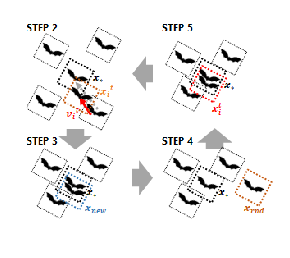
\includegraphics[width=1.0\linewidth]{eps/bbat_motion.eps}
% \end{center}
% \caption{Bat Motion of BA}
% \label{fig:bbat}
% \end{figure}

\begin{itemize}
\item STEP1: Initialize population of bats (line 1 to 3)\\
Initialize location ${x_i}(i=1, 2, ..., n)$ with velocity\\ ${v_i}(i=1, 2, ..., n)$ randomly. Each bat has loudness ${A_0}$, parse rate ${r_i}$ and frequency ${f_i}$ as initial value.
\item STEP2: Generate new solutions (line 6 to 7)\\
Generate new solutions ${x_i^t}$ based on equation (\ref{eq:xi}).
\item STEP3: In local search phase, Generate a new solution around global best solution ${x_*}$ (line 8 to 12)\\
In case of a random distribution higher than parse rate ${r_i}$, generate a new solution ${x_{new}}$ around ${x_*}$.
\item STEP4: Generate a new solution randomly (line 13)\\
Generate a new solution ${x_{rnd}}$ by random generation of bat.  
\item STEP5: Rank and update solutions (line 14 to 17)\\
In case of ${rand < A_i}$, choose the best from all solutions which are ${x_i, x_{new}}$, and ${x_{rnd}}$, and cross over as personal best solution unless it is higher than the value of former iteration.  
\item STEP6: Loop to STEP2 
\end{itemize}

\begin{algorithm}[H]
\caption{Bat Algorithm}
\label{code:ba}
\begin{algorithmic}[1]
\REQUIRE $Objective\ Function\ f(x)$
\STATE Initialize Population $x_i(i=1,2,..., n)$ and $v_i$\\
\STATE Define frequency $f_i$ at location $x_i$ \\
\STATE Initialize pulse rates $r_i$, and loudness $A_i$
\WHILE{($t <$ Max number of iterations)}
\FOR{i=1 to n}
\STATE Generate new solutions $x_i$ by tuning frequency $f_i$
\STATE Update location $x_i$ and velocity $v_i$  [eqs.(\ref{eq:freq}) to (\ref{eq:xi})]
\IF{($rand>r_i$)}
\STATE Generate a new solution $x_{new}$ around global best solution $x_i$ [eq.(\ref{eq:loc})] 
\ELSE
\STATE Continue
\ENDIF
\STATE Generate a new solution $x_{rnd}$ randomly
\IF{($rand<A_i \& {f(x_i), f(x_{new}), f(x_{rnd})}<f(x_*)$)}
\STATE Accept the new solution, and update pulse rate $r_i$ \\ \& loudness $A_i$ [eqs. (\ref{eq:A})(\ref{eq:r})]  
\ENDIF
\STATE Evaluate the all bats and select a best solution $x_*$ in the current solutions
\ENDFOR
\ENDWHILE
\end{algorithmic}
\end{algorithm}

\section{Distributed Bat Algorithm}
For reaching peaks of local minima and global minima located, we have to make bats spread widely. In k-nearest neighbor bat algorithm (k-NNBA), we focus on difference between the number of population. In Novelty Search-based bat algorithm (NSBA), we consider as written the difference above, and distance of each bat.
\subsection{k-Nearest Neighbor Bat Algorithm}
k-nearest neighbor (k-NN) method is used for classification for data with discrete label basically. The mechanism of k-nearest\\ neighbor is to find a new object (a new point) with closest distance between the other objects around it, and predict discrete label from these factors. Here, we use a new object as a new solution with the distance for keeping each bat away. The distance equation is written as below.

\begin{equation}
d_i^{t-1}=\cfrac{1}{K}\sum_{j=1}^K {(x_{i*}-x_j^{t-1})}
\label{eq:kd*}
\end{equation}
\begin{equation}
d_i^{t-1}=\cfrac{1}{K}\sum_{j=1}^K {(x_i^{t-1}-x_j^{t-1})}
\label{eq:kdi}
\end{equation}

K describes the number of nearest neighbor. In equation (\ref{eq:nd*}), ${x_{i*}}$ means personal best solution. k-NN is very simple method and is easy to implement, but depending on number of neighbors, we have to choose proper k. Pseudo code is described in Algorithm 2.

\subsection{Novelty Search-based Bat Algorithm}
\subsubsection{Novelty Search}
Novelty search is used as evolutionary search approach to expand dense solutions into sparse area and to measure the distance between current solutions to reward or delete it. The sparseness of solutions is calculated as below,
\begin{equation}
\rho(x)=\cfrac{1}{k}\sum_{i=0}^k dist(x,\mu_i),
\label{eq:nov}
\end{equation}
where the sparseness ${\rho(x)}$ at a point ${x}$ shows the scatter of solutions. The dist in k-nearest neighbors is the average distance between the point ${x}$ and ${\mu_i}$, which is the ${i}$th nearest neighbor of ${x}$. 
% This is an example in case of k neighbor = 3 (shown in Fig. \ref{fig:n_dist}). It describes that a solution is migrated away from three neighbors. 

% \begin{figure}[h]
% \begin{center}
% 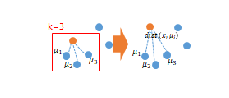
\includegraphics[width=1.0\linewidth]{eps/n_dist.eps}
% \end{center}
% \caption{distributed a solution to sparse area}
% \label{fig:n_dist}
% \end{figure}

\subsubsection{Novelty Search-based Bat Algorithm}
In order to adapt multimodal optimization not only single objective optimization, Novelty Search-based Bat Algorithm (NSBA) enables all population to reach local minima. This paper proposes a method of keeping over a certain distance between each location of bat, and letting population remain around local minima. Using this behavior, all population are updated by the equation as bellow, 
\begin{equation}
d_i^{t-1}=\cfrac{1}{K}\sum_{j=1}^K \cfrac{(x_{i*}-x_j^{t-1})}{|x_{i*}-x_j^{t-1}|^2}
\label{eq:nd*}
\end{equation}
\begin{equation}
d_i^{t-1}=\cfrac{1}{K}\sum_{j=1}^K \cfrac{(x_i^{t-1}-x_j^{t-1})}{|x_i^{t-1}-x_j^{t-1}|^2}
\label{eq:ndi}
\end{equation}

where ${K}$ is population size of nearest neighbor, and ${x_{i*}}$ indicates personal best solution. ${x_i^{t-1}}$ is previous position of solution. In addition, bats with velocity ${v_i^t}$ and location ${x_i^t}$ are updated same as (\ref{eq:vel}) and (\ref{eq:xi}) of conventional method. Used distance function in Novelty search describes scalar equation. However in this proposes, we alter scalar to vector equation for determining search direction. 

 \subsubsection{Distance of each bat} 
 Above-mentioned the vector equation \ref{eq:kd*} and \ref{eq:kdi}, as distance of each bat is closer, they hardly move to sparse area. Conversely, as they located far away each other, they move greatly up to a boundary of search area. To control this movement, we introduce the denominator as equation (\ref{eq:nd*})(\ref{eq:ndi}). Here is the Algorithm flow on global minimum optimization. The NSBA pseudo code is described in Algorithm 2.

\begin{itemize}
\item STEP1: Initialize population of bats (line 1 to 3)\\
Initialize location ${x_i}(i=1, 2, ..., n)$ with velocity\\ ${v_i}(i=1, 2, ..., n)$ randomly. Each bat has loudness ${A_0}$, parse rate ${r_i}$ and frequency ${f_i}$ as initial value.
\item STEP2: Generate new solutions (line 6 to 7)\\
Generate new solutions ${x_i^t}$ based on equation (\ref{eq:vel})(\ref{eq:xi}) with (\ref{eq:ndi}) or (\ref{eq:nd*}).
\item STEP3: In local search phase, Generate a new solution around solutions ${x_i}$ (line 8 to 12)\\
In case of a random distribution higher than parse rate ${r_i}$, generate a new solution ${x_{local}}$ around ${x_i}$.
\item STEP4: Generate a new solution randomly (line 13)\\
Generate a new solution ${x_{rnd}}$ by random walk of bat.  
\item STEP5: Rank and update solutions (line 14 to 18)\\
If ${rand < A_i}$, choose the best from all solutions which are ${x_i, x_{local}}$, and ${x_{rnd}}$. After that, cross over as personal best solution unless it is higher fitness value than previous iteration.  
\item STEP6: Loop to STEP2
\end{itemize}

\begin{figure}[h]
\begin{center}
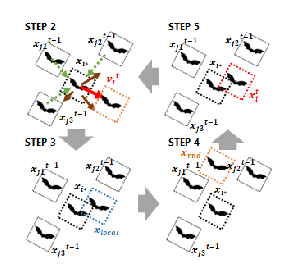
\includegraphics[width=0.8\linewidth]{eps/sbat_motion.eps}
\end{center}
\caption{Bat motion of NSBA}
\label{fig:sbat}
\end{figure}

\begin{algorithm}[H]
\caption{Distributed Bat Algorithm}
\label{code:sba}
\begin{algorithmic}[1]
\REQUIRE $Objective\ Function\ f(x)$
\STATE Initialize Population $x_i(i=1,2,..., n)$ and $v_i$\\
\STATE Define frequency $f_i$ at location $x_i$ \\
\STATE Initialize pulse rates $r_i$, and loudness $A_i$
\WHILE{($t <$ Max number of iterations)}
\FOR{i=1 to n}
\STATE Generate new solutions $x_i$ by tuning frequency $f_i$
\STATE Update location $x_i$, velocity $v_i$  [eqs.(\ref{eq:freq})(\ref{eq:vel})(\ref{eq:xi})] \\ and k-NNBA for [eq.(\ref{eq:kd*})(\ref{eq:kdi})] NSBA for [eq.(\ref{eq:nd*})(\ref{eq:ndi})] 
\IF{($rand>r_i$)}
\STATE Generate a new solution ${x_{local}}$ around the solution $x_{i}$ [eq.(\ref{eq:loc})] 
\ELSE
\STATE Continue
\ENDIF
\STATE Generate a new solution $x_{rnd}$ randomly (or without ${x_{rnd}}$)
\IF{($rand<A_i \& f(x_i)<f(x_i)$)}
\STATE Accept the new solution, and update pulse rate $r_i$ \\ \& loudness $A_i$ [eqs. (\ref{eq:A})(\ref{eq:r})]  
\ENDIF
\ENDFOR
\STATE Evaluate the all bats and select a best solution $x_i*$ in the current solutions
\ENDWHILE
\end{algorithmic}
\end{algorithm}

\subsection{Comparion with k-NNBA and NSBA}
we compare 8 methods in total. There are comparison of these methods on below Table \ref{tb:compare}.  
\begin{table}[h]
\begin{center}
\caption{Comparion with k-NNBA \& NSBA}
\label{tb:compare}
\begin{tabular}{c|c|c|c|c}
\hline 
\multicolumn{1}{c|}{${x_{rnd}}$} & \multicolumn{2}{c|}{$\circ$} & \multicolumn{2}{c}{$\times$}   \\
\hline
 x & ${x_{i*}}$ & ${x_i^{t-1}}$ & ${x_{i*}}$ & ${x_i^{t-1}}$ \\
\hline 
k-NNBA & I & II & III & IV\\
NSBA & V & VI & VII & VIII\\
\hline
\end{tabular}
\end{center}
\end{table}

\section{Multimodal Function}
 In the contour of function, there are the coordinate that horizontal axis is x1 and vertical axis is x2, and the colorbar that color density describes the fitness value shown as Fig. \ref{fig:cf}. As color becomes darker area, fitness value gets lower. For validating NSBA to distribute spread widely, there are some multimodal functions. Focused on depth of fitness value, scale of multimodal domain and number of local minima, we used these functions as following section.  
\subsection{Griewank Function}
As an example to demonstrate the bat motion of this algorithm, we use Griewank function as below (shown in Fig. \ref{fig:3dgf})
\begin{equation}
f(x)= \sum_{i=1}^d \cfrac{x_{i}}{4000} - \prod_{i=1}^d \cos(\cfrac{x_i}{\sqrt{i}}) + 1,
\end{equation}
where global optimum is ${f(x_*)}=0$, at $x_* = {[0 \ \ 0]}$. There are 17 local minima at ${\pm x \approx}$ ${ [6.2800 \ \ 8.8769],}$ ${[3.1400 \ \ 4.4385],}$ \\ ${[0 \ \ 8.8769]}$, ${[6.2800 \ \ 0], [9.4200 \ \ 4.4385]}$ in the range of this function is between ${-10 \leq x_i \leq 10}$ with i=1,2,...,d. The function ${f(x)}$ has global minimum ${f(x_*)}=0$ and also the other local minima ${f(x_{i*)} \approx 0}$  for ${d=2}$.  

 \subsection{Rastrigin Function}
 This function has 121 local minima in the spatial domain, at ${ \pm x=}$ ${[0,...,11 \ \ 0,...,11]}$. And global minimum is ${f(x_*)=0}$ at ${x=[0 \ \ 0]}$. The function equation is
 \begin{equation}
f(x)= 10d+\sum_{i=1}^d [x_i^2-10 \cos(2\pi x_i)]
\end{equation}
3D model and contour of this function are showed in Fig. \ref{fig:3drf} \& \ref{fig:rfc}. 

% \subsection{Eggholder function}
%  There are uncountable local minima in this function due to complex equation as below.
%  \begin{equation}
% f(x)= -(x_2+47) \sin (\sqrt{|x_2+\cfrac{x_1}{2}+47|})-x_1\sin(\sqrt{|x_1-(x_2+47)|})
% \end{equation}
% Global minimum is ${f(x_*)}=-959.64$ at ${x_*}=[512 \ \ 404.23]$. The graph of this function shows in Fig. \ref{fig:3def}.

\begin{figure}[h]
\centering
\subfigure[Griewank function]{
\includegraphics[width=0.9\linewidth]{eps/Griewank.eps}
\label{fig:3dgf}}
\subfigure[Rastrigin function]{
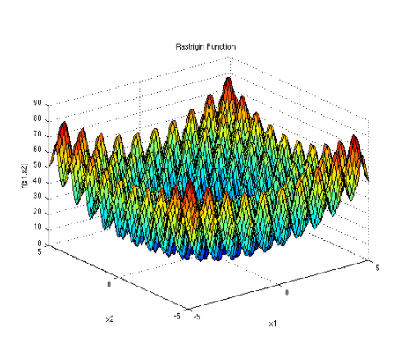
\includegraphics[width=0.8\linewidth]{eps/rastrigin.eps}
\label{fig:3drf}}

\caption{3D model Function}
\label{fig:3d}
\end{figure}

\begin{figure}[h]
\centering
\subfigure[Griewank function]{
\includegraphics[width=0.8\linewidth]{eps/Griewank_cont.eps}
\label{fig:gfc}}
\subfigure[Rastrigin function]{
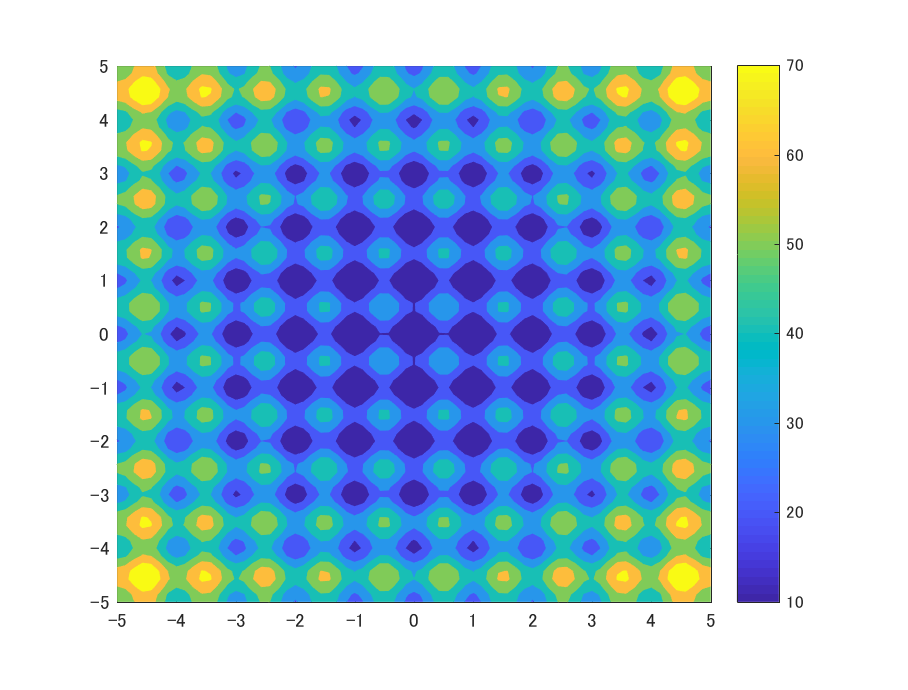
\includegraphics[width=0.8\linewidth]{eps/rastrigin_cont.eps}
\label{fig:rfc}}

\caption{Contour of Functions}
\label{fig:cf}
\end{figure}

\section{Experiment}
 We compared proposed NSBA with the other algorithms, which NNBA and BA. Each algorithm was run for 10 seeds to validate the performance of NSBA. In this paper, the algorithm is implemented on MATLAB for the benchmark function.

\subsection{Evaluation Criteria}
$dist$ is total amount of the distance between local minima and nearest neighbor population, in case of initializing population randomly each algorithm. In this experiment, we focus on how many found local minima, and $dist$ which total amount of the distance between local minima and the closest solutions, as below. \\
\begin{equation}
dist=\sum_{i=1}^M {min_{j \in N}|s_i-x_j|},
\label{eq:dist}
\end{equation}
 where ${M}$ is maximum number of local minimum, and ${N}$ is population size of bats. ${s_i}$ means the coordinate of local minimum. As ${dist}$ is closed zero, the number of bats located local minima increases. We compare with the performance of these algorithms in term of the population size and the bat behavior by iteration. 

\subsection{Experimental Parameter}
All experiments use same parameters, where population size\\ ${N=20}$, frequency ${f_{max}=1, f_{min}=0}$, loudness ${A^0}=1$, parse rate ${r^0} \in [0 \ \ 1]$ with ${\alpha =\gamma = 0.9}$.

\subsection{Result}
 \subsubsection{Comparison with I and V}
On griewank function, dist of k-NNBA and NSBA are nearly same in any neighbors, but k-NNBA is slightly better performance than NSBA on each function. From rastrigin function, k-NNBA is smaller than NSBA in any neighbors.

\subsubsection{Comparison with II and VI}
On griewank function, NSBA is almost better than k-NNBA in each neighbor except for K=4, dist of k-NNBA is a bit smaller. Overall, ${dist}$ is higher than the other methods on griewank function. In rastrigin function, k-NNBA gradually increased. However, NSBA slowly decreased until K=16.

\subsubsection{Comparison with III and VII}
Method III and VII are better performance than the other mothods in griewank function.
However, k-NNBA became worse as increasing neighbors. By contrast, NSBA was very unchanged in any neighbors. Besides, averages of k-NNBA and NSBA almost unchanged.  

 \subsubsection{Comparison with IV and VIII}
The dist of NSBA is smaller than k-NNBA in K=2 to 20 on both functions, except for K=2 and 4 on rastrigin function. The average of NSBA also smaller than k-NNBA. 
 Comparison to NSBA in Fig. \ref{fig:*bar_func}, dist of k-NNBA is lowest of the other number of neighbors. However, dist of k-NNBA rose up gradually from K=4. By contrast, dist of NSBA remains fairly on griewank function, but the performance gets worse after K=4. Overall, 

\begin{figure*}[p]
\centering
\begin{tabular}{c}
\begin{minipage}{0.49\hsize}
\centering
\subfigure[Griewank Function]{
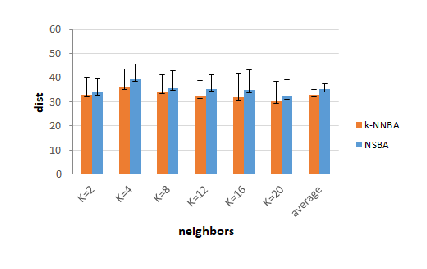
\includegraphics[width=1.0\textwidth]{eps/pbest_grie_r.eps}
\label{fig:r*bar_grie}}
\end{minipage}
\begin{minipage}{0.49\hsize}
\centering
\subfigure[Rastrigin Function]{
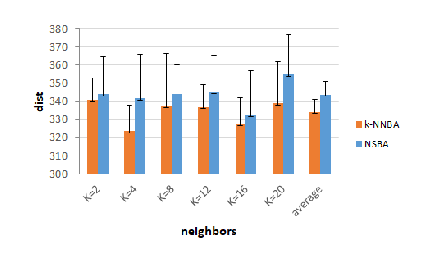
\includegraphics[width=1.0\textwidth]{eps/pbest_rast_r.eps}
\label{fig:r*bar_rast}}
\end{minipage}
\end{tabular}
\label{fig:r*bar_func}
\caption{Comparison with method I \& V}
\end{figure*}

\begin{figure*}[p]
\centering
\begin{tabular}{c}
\begin{minipage}{0.49\hsize}
\centering
\subfigure[Griewank Function]{
\includegraphics[width=1.0\textwidth]{eps/t-1_grie_r.eps}
\label{fig:rtbar_grie}}
\end{minipage}
\begin{minipage}{0.49\hsize}
\centering
\subfigure[Rastrigin Function]{
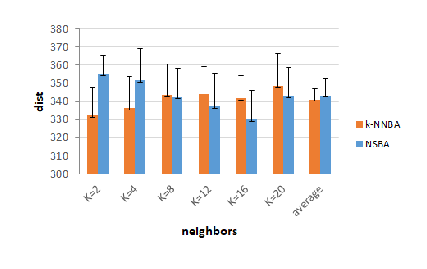
\includegraphics[width=1.0\textwidth]{eps/t-1_rast_r.eps}
\label{fig:rtbar_rast}}
\end{minipage}
\end{tabular}
\caption{Comparison with method II \& VI}
\label{fig:rtbar_func}
\end{figure*}

\begin{figure*}[p]
\centering
\begin{tabular}{c}
\begin{minipage}{0.49\hsize}
\centering
\subfigure[Griewank Function]{
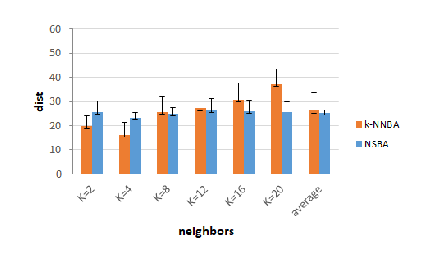
\includegraphics[width=1.0\textwidth]{eps/pbest_grie.eps}
\label{fig:*bar_grie}}
\end{minipage}
\begin{minipage}{0.49\hsize}
\centering
\subfigure[Rastrigin Function]{
\includegraphics[width=1.0\textwidth]{eps/pbest_rast.eps}
\label{fig:r*bar_rast}}
\end{minipage}
\end{tabular}
\caption{Comparison with method III \& VII}
\label{fig:*bar_func}
\end{figure*}

\begin{figure*}[p]
\centering
\begin{tabular}{c}
\begin{minipage}{0.49\hsize}
\centering
\subfigure[Griewank Function]{
\includegraphics[width=1.0\textwidth]{eps/t-1_grie.eps}
\label{fig:tbar_grie}}
\end{minipage}
\begin{minipage}{0.49\hsize}
\centering
\subfigure[Rastrigin Function]{
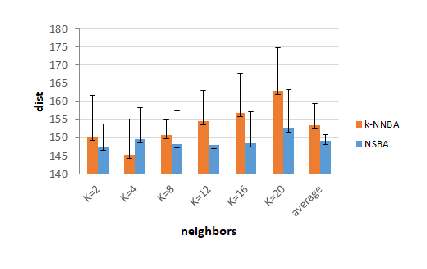
\includegraphics[width=1.0\textwidth]{eps/t-1_rast.eps}
\label{fig:rtbar_rast}}
\end{minipage}
\end{tabular}
\caption{Comparison with method IV \& VIII}
\label{fig:tbar_func}
\end{figure*}

%%%%%%%%%%%%%%%%%%%%%%%%%%%%%%%%%%%%%%%%%%%%%%%%%%%%%%%%%%%%%%%
% \begin{figure}[p]
% \centering
% \subfigure[Griewank Function]{
% 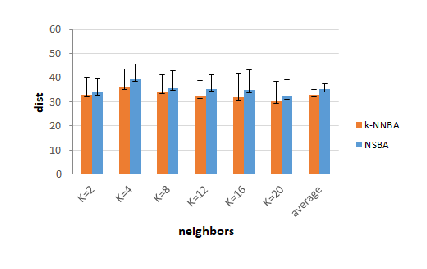
\includegraphics[width=0.4\textwidth]{eps/pbest_grie_r.eps}
% \label{fig:r*bar_grie}}

% \subfigure[Rastrigin Function]{
% 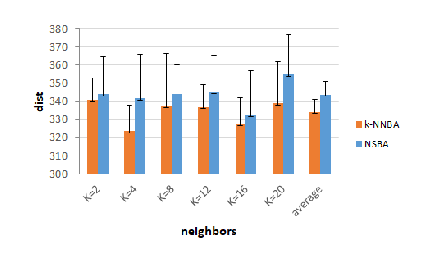
\includegraphics[width=0.4\textwidth]{eps/pbest_rast_r.eps}
% \label{fig:r*bar_rast}}
% \caption{Comparison with method I \& V}
% \label{fig:r*bar_func}
% \end{figure}

% \begin{figure}[p]
% \centering
% \subfigure[Griewank Function]{
% \includegraphics[width=0.4\textwidth]{eps/t-1_grie_r.eps}
% \label{fig:rtbar_grie}}

% \subfigure[Rastrigin Function]{
% 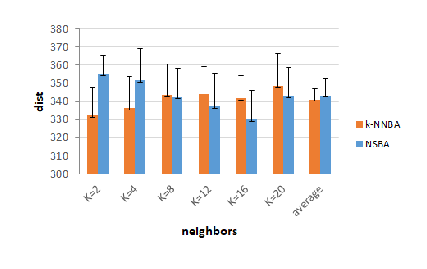
\includegraphics[width=0.4\textwidth]{eps/t-1_rast_r.eps}
% \label{fig:rtbar_rast}}
% \caption{Comparison with method II \& VI}
% \label{fig:rtbar_func}
% \end{figure}

% \begin{figure}[p]
% \centering
% \subfigure[Griewank Function]{
% 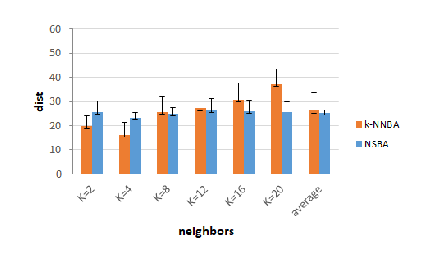
\includegraphics[width=0.4\textwidth]{eps/pbest_grie.eps}
% \label{fig:*bar_grie}}

% \subfigure[Rastrigin Function]{
% \includegraphics[width=0.4\textwidth]{eps/pbest_rast.eps}
% \label{fig:r*bar_rast}}
% \caption{Comparison with method III \& VII}
% \label{fig:*bar_func}
% \end{figure}

% \begin{figure}[p]
% \centering
% \subfigure[Griewank Function]{
% \includegraphics[width=0.4\textwidth]{eps/t-1_grie.eps}
% \label{fig:tbar_grie}}

% \subfigure[Rastrigin Function]{
% 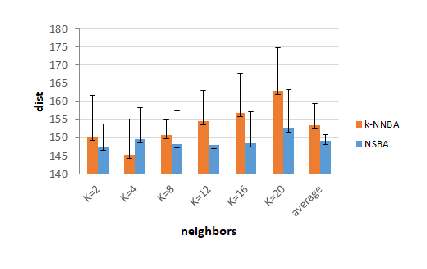
\includegraphics[width=0.4\textwidth]{eps/t-1_rast.eps}
% \label{fig:rtbar_rast}}
% \caption{Comparison with method IV \& VIII}
% \label{fig:tbar_func}
% \end{figure}

\begin{figure*}[p]
\centering
\begin{tabular}{c}
\begin{minipage}{0.49\hsize}
\centering
\subfigure[k-NNBA]{
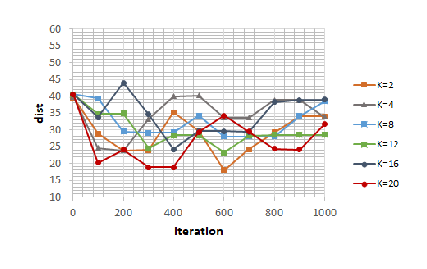
\includegraphics[width=1.0\textwidth]{eps/ip_k_r.eps}
\label{fig:ri*_k}}
\end{minipage}
\begin{minipage}{0.49\hsize}
\centering
\subfigure[NSBA]{
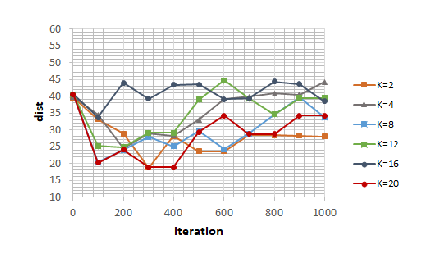
\includegraphics[width=1.0\textwidth]{eps/ip_ns_r.eps}
\label{fig:ri*_ns}}
\end{minipage}
\end{tabular}
\caption{Comparison with method I \& V}
\label{fig:ri*_iter}
\end{figure*}

\begin{figure*}[p]
\centering
\begin{tabular}{c}
\begin{minipage}{0.49\hsize}
\centering
\subfigure[k-NNBA]{
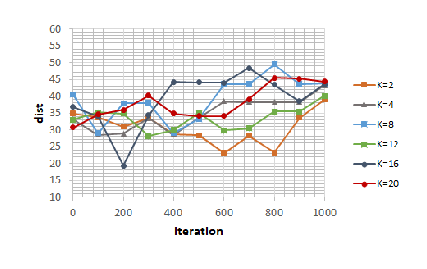
\includegraphics[width=1.0\textwidth]{eps/it-1_k_r.eps}
\label{fig:rit_k}}
\end{minipage}
\begin{minipage}{0.49\hsize}
\centering
\subfigure[NSBA]{
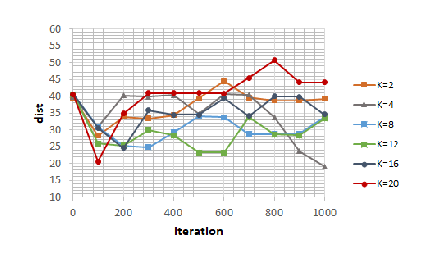
\includegraphics[width=1.0\textwidth]{eps/it-1_ns_r.eps}
\label{fig:rit_ns}}
\end{minipage}
\end{tabular}
\caption{Comparison with method II \& VI}
\label{fig:rit_iter}
\end{figure*}

\begin{figure*}[p]
\centering
\begin{tabular}{c}
\begin{minipage}{0.49\hsize}
\centering
\subfigure[k-NNBA]{
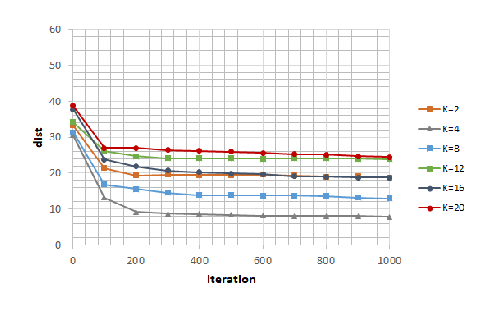
\includegraphics[width=1.0\textwidth]{eps/ip_k.eps}
\label{fig:i*_k}}
\end{minipage}
\begin{minipage}{0.49\hsize}
\centering
\subfigure[NSBA]{
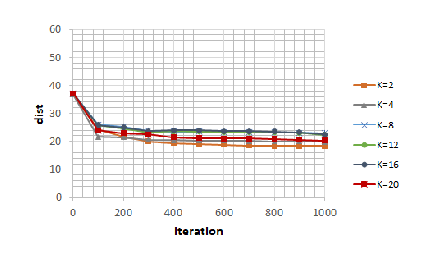
\includegraphics[width=1.0\textwidth]{eps/ip_ns.eps}
\label{fig:i*_ns}}
\end{minipage}
\end{tabular}
\caption{Comparison with method III \& VII}
\label{fig:i*_iter}
\end{figure*}

\begin{figure*}[p]
\centering
\begin{tabular}{c}
\begin{minipage}{0.49\hsize}
\centering
\subfigure[k-NNBA]{
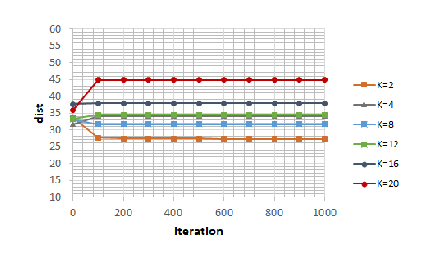
\includegraphics[width=1.0\textwidth]{eps/it-1_k.eps}
\label{fig:it_k}}
\end{minipage}
\begin{minipage}{0.49\hsize}
\centering
\subfigure[NSBA]{
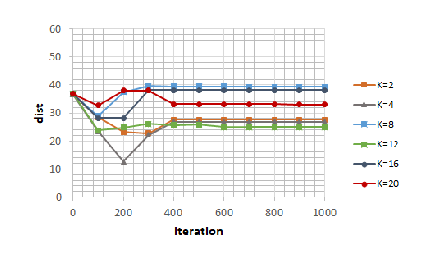
\includegraphics[width=1.0\textwidth]{eps/it-1_ns.eps}
\label{fig:it_ns}}
\end{minipage}
\end{tabular}
\caption{Comparison with method IV \& VIII}
\label{fig:it_iter}
\end{figure*}

% \begin{figure}[p]
% \centering
% \subfigure[k-NNBA]{
% 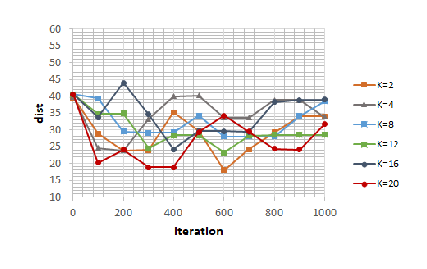
\includegraphics[width=0.4\textwidth]{eps/ip_k_r.eps}
% \label{fig:ri*_k}}

% \subfigure[NSBA]{
% 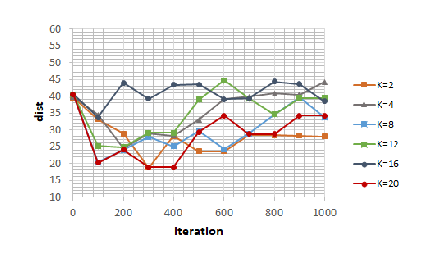
\includegraphics[width=0.4\textwidth]{eps/ip_ns_r.eps}
% \label{fig:ri*_ns}}
% \caption{Comparison with method I \& V}
% \label{fig:ri*_iter}
% \end{figure}

% \begin{figure}[p]
% \centering
% \subfigure[k-NNBA]{
% 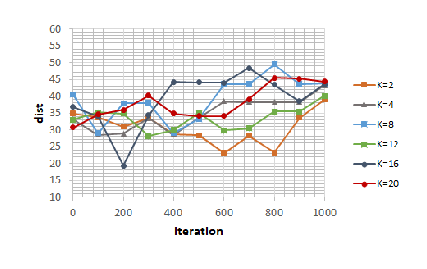
\includegraphics[width=0.4\textwidth]{eps/it-1_k_r.eps}
% \label{fig:rit_k}}

% \subfigure[NSBA]{
% 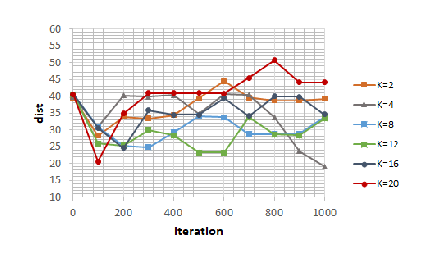
\includegraphics[width=0.4\textwidth]{eps/it-1_ns_r.eps}
% \label{fig:rit_ns}}
% \caption{Comparison with method II \& VI}
% \label{fig:rit_iter}
% \end{figure}

% \begin{figure}[p]
% \centering
% \subfigure[k-NNBA]{
% 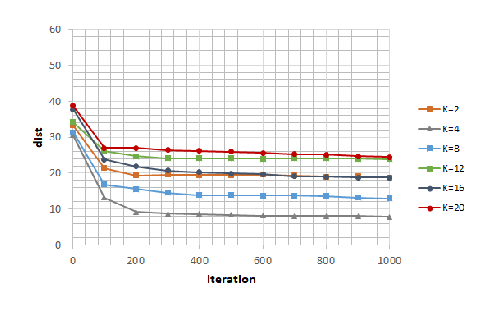
\includegraphics[width=0.46\textwidth]{eps/ip_k.eps}
% \label{fig:i*_k}}

% \subfigure[NSBA]{
% 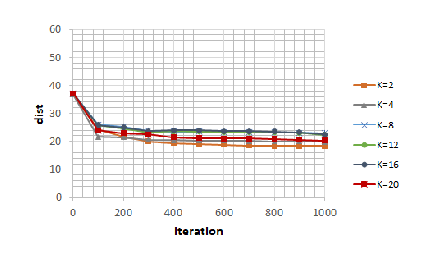
\includegraphics[width=0.47\textwidth]{eps/ip_ns.eps}
% \label{fig:i*_ns}}
% \caption{Comparison with method III \& VII}
% \label{fig:i*_iter}
% \end{figure}

% \begin{figure}[p]
% \centering
% \subfigure[k-NNBA]{
% 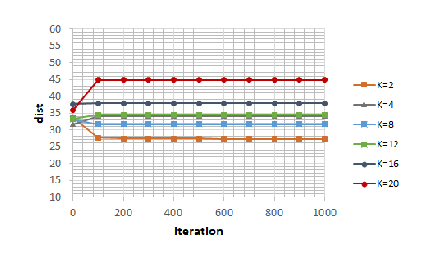
\includegraphics[width=0.46\textwidth]{eps/it-1_k.eps}
% \label{fig:it_k}}

% \subfigure[NSBA]{
% 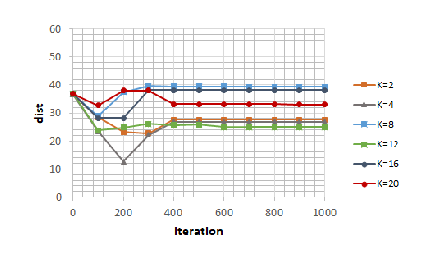
\includegraphics[width=0.46\textwidth]{eps/it-1_ns.eps}
% \label{fig:it_ns}}
% \caption{Comparison with method IV \& VIII}
% \label{fig:it_iter}
% \end{figure}

% \begin{figure}[p]
% \begin{center}
% \begin{tabular}{c}
% \begin{minipage}{0.49\hsize}
%   \begin{center}
%    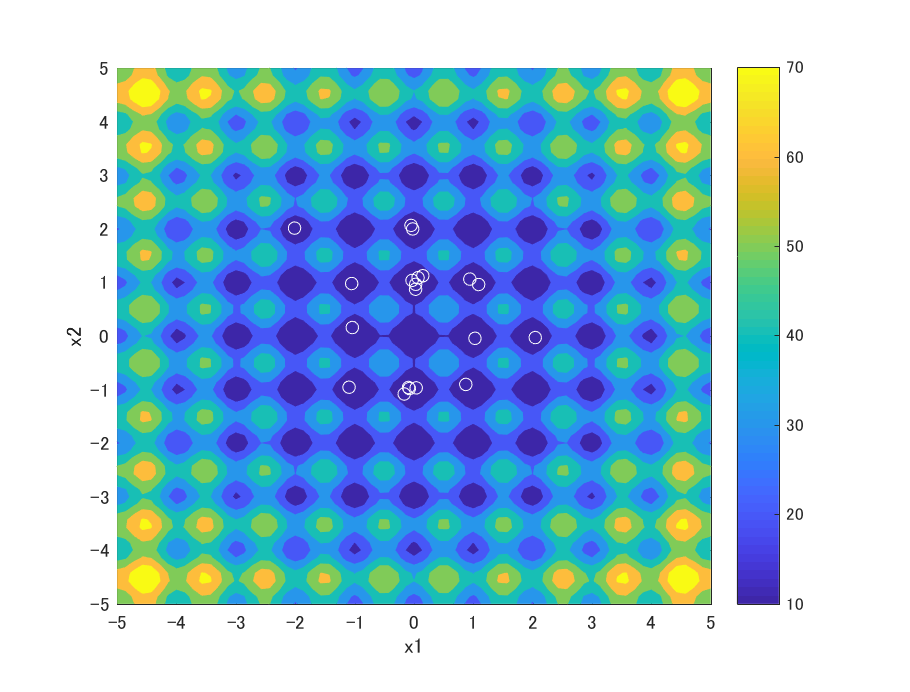
\includegraphics[width=45mm]{eps/i_k=4_1000.eps}
%    \hspace{1.0cm} (a) k-NNBA
%   \end{center}
%   \label{fig:_k=4_i}
%  \end{minipage}

%  \begin{minipage}{0.49\hsize}
%   \begin{center}
%    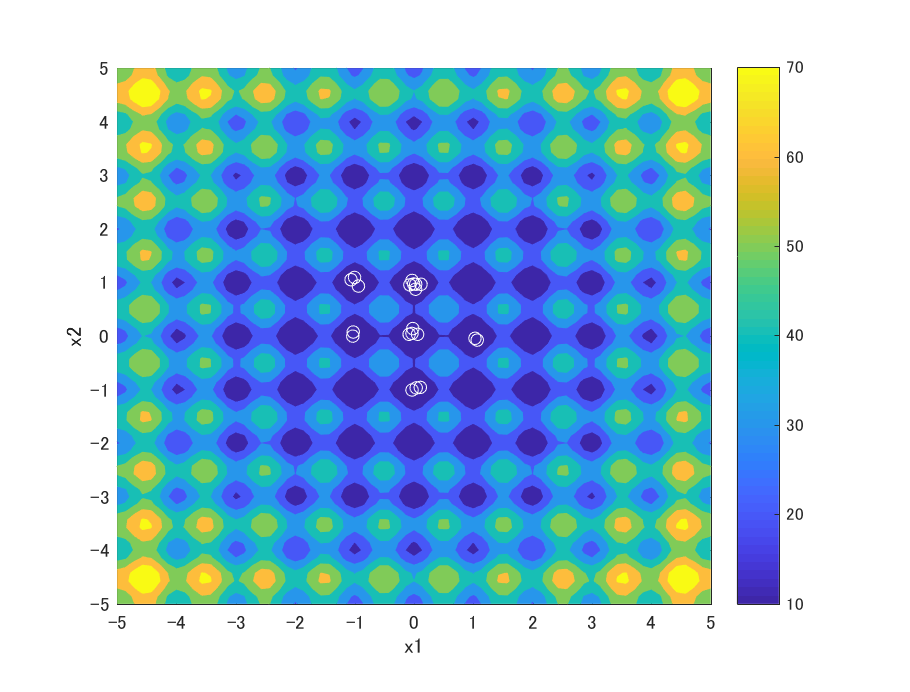
\includegraphics[width=45mm]{eps/v_k=4_1000.eps}
%    \hspace{1.0cm} (b) NSBA
%   \end{center}
%   \label{fig:k=4_v}
%  \end{minipage}
% \end{tabular}
% \end{center}
% \caption{method I \& V (K=4)}
% \label{fig:1000_15}
% \end{figure}

% \begin{figure}[p]
% \begin{center}
% \begin{tabular}{c}
% \begin{minipage}{0.49\hsize}
%   \begin{center}
%    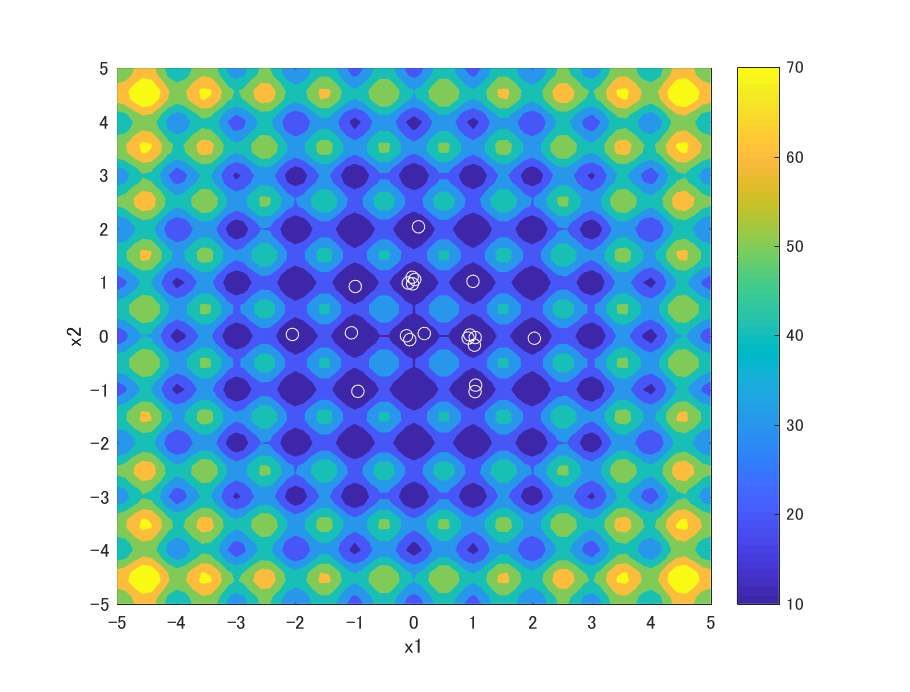
\includegraphics[width=45mm]{eps/ii_k=4_1000.eps}
%    \hspace{1.0cm} (a) k-NNBA
%   \end{center}
%   \label{fig:k=4_ii}
%  \end{minipage}

%  \begin{minipage}{0.49\hsize}
%   \begin{center}
%    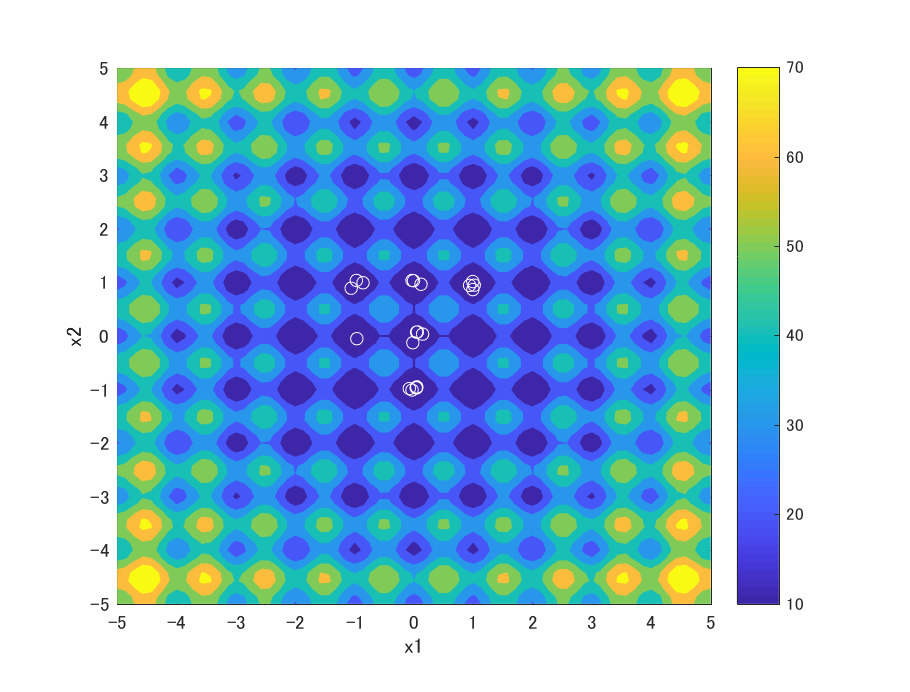
\includegraphics[width=45mm]{eps/vi_k=4_1000.eps}
%    \hspace{1.0cm} (b) NSBA
%   \end{center}
%   \label{fig:k=4_vi}
%  \end{minipage}
% \end{tabular}
% \end{center}
% \caption{method II \& VI (K=4)}
% \label{fig:1000_26}
% \end{figure}

% \begin{figure}[p]
%   \begin{center}
% \begin{tabular}{c}
% \begin{minipage}{0.49\hsize}
%   \begin{center}
%    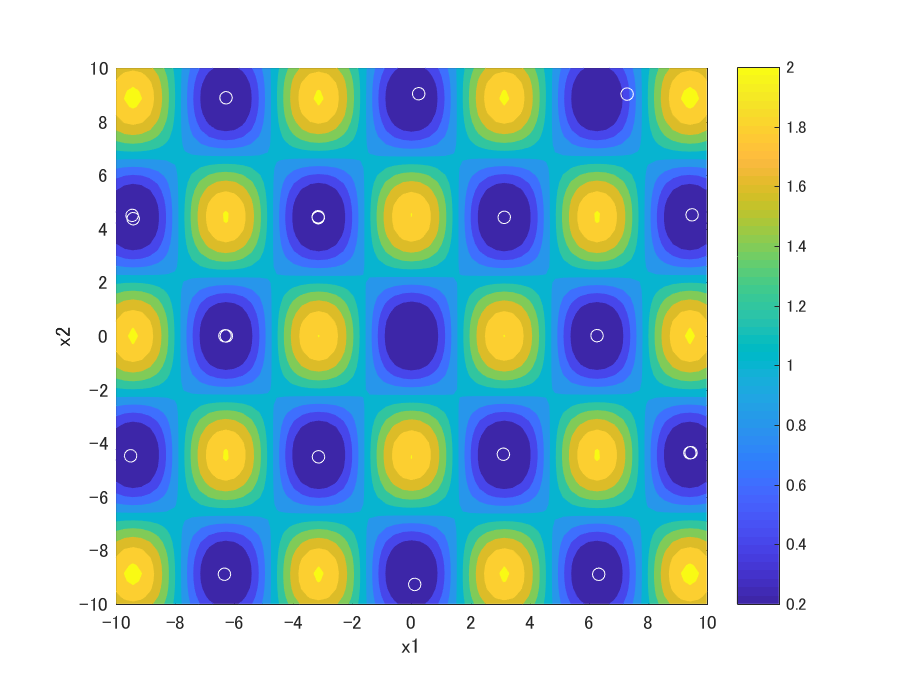
\includegraphics[width=45mm]{eps/iii_k=4_1000.eps}
%    \hspace{1.0cm} (a) k-NNBA
%   \end{center}
%   \label{fig:k=4_iii}
%  \end{minipage}

%  \begin{minipage}{0.49\hsize}
%   \begin{center}
%    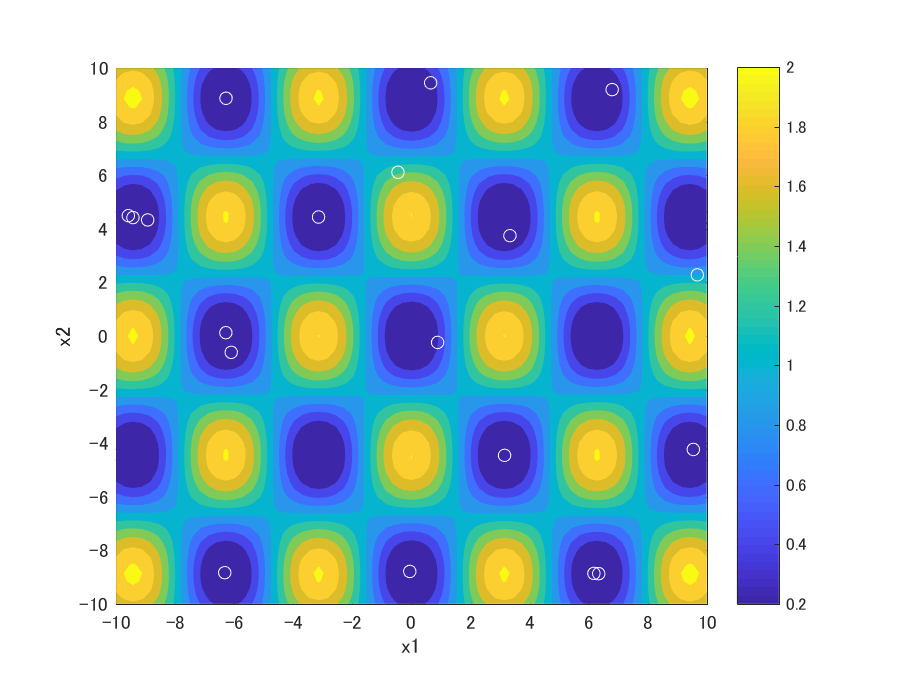
\includegraphics[width=45mm]{eps/vii_k=4_1000.eps}
%    \hspace{1.0cm} (b) NSBA
%   \end{center}
%   \label{fig:k=4_vii}
%  \end{minipage}

% \end{tabular}
% \caption{method III \& VII (K=4)}
% \label{fig:1000_37}
% \end{center}
% \end{figure}

% \begin{figure}[p]
% \begin{center}
% \begin{tabular}{c}
% \begin{minipage}{0.49\hsize}
%   \begin{center}
%    \includegraphics[width=45mm]{eps/iv_k=4_1000.eps}
%    \hspace{1.0cm} (a) k-NNBA
%   \end{center}
%   \label{fig:k=4_iv}
%  \end{minipage}

%  \begin{minipage}{0.49\hsize}
%   \begin{center}
%    \includegraphics[width=45mm]{eps/viii_k=4_1000.eps}
%    \hspace{1.0cm} (b) NSBA
%   \end{center}
%   \label{fig:k=4_viii}
%  \end{minipage}
% \end{tabular}
% \end{center}
% \caption{method IV \& VIII (K=4)}
% \label{fig:1000_48}
% \end{figure}


\section{Discussion}
There are line graphs for all methods on Griewank function. The horizontal axis describes iteration of evaluating solutions, and vertical axis describes the sum of distance between each local minima and the closest solution shown as Fig. \ref{fig:ri*_iter} to \ref{fig:it_iter}.
 % Besides distributed solutions at 1000th iteration step from Fig. \ref{fig:1000_15} and \ref{fig:1000_26} for rastrigin function from Fig. \ref{fig:1000_37} and \ref{fig:1000_48} for griewank function. 
\subsection{k-NNBA vs NSBA}
From Fig. \ref{fig:rtbar_func} to \ref{fig:tbar_func}, k-NNBA tends to decline as neighbors increase. NSBA is hardly affected by changes of neighbors, so that it performed better than k-NNBA relatively. 
% Especially in k=4 from Fig. \ref{fig:1000_15}, \ref{fig:1000_26} and \ref{fig:1000_48}, k-NNBA more distributed than NSBA obviously. It means that equation of considering distance still performed weakly.
 For this reason, we have to adjust the number of neighbors and population size and updating equation.
  
\subsection{Existence or nonexistence of ${x_{rnd}}$}
Compared line graph with Fig. \ref{fig:ri*_iter} \& \ref{fig:rit_iter} and Fig. \ref{fig:i*_iter} \& \ref{fig:it_iter}, ${x_{rnd}}$ affected iteration step. Especially in Fig. \ref{fig:ri*_iter} \& \ref{fig:it_iter}, ${dist}$ fluctuated until 1000 iteration steps in any neighbors. By contrast in Fig. \ref{fig:i*_iter} \& \ref{fig:it_iter}, ${dist}$ of any neighbors became stable over a certain iteration. 

\subsection{Differences in ${x_i^{t-1}}$ and ${x_{i*}}$}
Focused on 4 line graphs in right side Fig. \ref{fig:i*_iter} and \ref{fig:it_iter} without ${s_{rnd}}$, ${x_{i*}}$ indicates personal best solution, these ${dist}$ fell continuously until 300 iterations and became stable to the end. From left side in Fig. \ref{fig:ri*_iter} \& \ref{fig:rit_iter}, all ${dist}$ fluctuated constantly, as ${x_{rnd}}$ has strong effect on iteration.


% \subsection{Different Population Size}
\begin{table}[h]
\begin{center}
\caption{$dist$ of NSBA}
\label{tb:nsba}
\begin{tabular}{cccc}
\hline 
Seed & $n=10$ & $n=20$ & $n=40$ 
\\
\hline \hline
1 & 57.89055 & 34.73127 & 36.01941 \\
2 & 74.33342 & 36.39555 & 17.5624 \\
3 & 58.77926 & 39.05099 & 28.25238 \\
4 & 55.87579 & 23.77053 & 17.093489 \\
5 & 62.14158 & 34.53509 & 17.76876 \\
6 & 49.07995 & 39.75885 & 22.30472 \\
7 & 53.441226 & 43.40263 & 12.50444 \\
8 & 65.24583 & 39.37115 & 28.42639 \\
9 & 65.17686 & 39.149967 & 22.16795 \\
10 & 64.97366 & 29.06209 & 22.04256 \\
\hline
Average & 60.6938 & 35.9228 & 22.4143 \\
SD & 7.22257 & 5.783791 & 6.889419 \\
\hline
\end{tabular}
\end{center}
\end{table}

% \begin{table}[h]
% \begin{center}
% \caption{the number of reached local minima}
% \label{tb:numsolp}
% \begin{tabular}{cccc}

% \hline
% & $n=10$ & $n=20$ & $n=40$
% \\
% \hline \hline
% average & 6 & 9.1 & 12.7 \\
% search ratio & 35.30 \% & 53.53 \% & 74.71 \% \\
% SD & 1.247219 & 0.875595 & 1.766981 \\
% \hline
% \end{tabular}
% \end{center}
% \end{table}

% We can see $dist$ was directly proportional to increase population size from Table. \ref{tb:nsba}, \ref{tb:numsolp}. Likewise SD gradually grew between $n=10$ to $40$. $dist$ was a significant rise from $n=20$ to $40$. 

  
\section{Conclusion}
We validated the performance of proposed bat algorithms for k-nearest neighbor and novelty search with changes of updating solutions and generating a new solution randomly. As a result, both algorithms performed for reaching local minima with global optimum. Especially the method using personal best without ${s_{rnd}}$, performed better than the other proposed methods. However, we have to adjust the number of neighbors for feasible multimodal functions. As population size of bat increases, the number of\\ searched local minima  also increased. Our future prospects are adapting this algorithm for the other benchmark functions, and blushing up the performance to cover unspecified large number of local minima. Future experiments on the other multimodal functions and investigation will be studied.


%\end{document}  % This is where a 'short' article might terminate


\appendix
%Appendix A
% \section{Headings in Appendices}
% The rules about hierarchical headings discussed above for
% the body of the article are different in the appendices.
% In the \textbf{appendix} environment, the command
% \textbf{section} is used to
% indicate the start of each Appendix, with alphabetic order
% designation (i.e., the first is A, the second B, etc.) and
% a title (if you include one).  So, if you need
% hierarchical structure
% \textit{within} an Appendix, start with \textbf{subsection} as the
% highest level. Here is an outline of the body of this
% document in Appendix-appropriate form:
% \subsection{Introduction}
% \subsection{Bat Algorithm}
% \subsubsection{Type Changes and  Special Characters}
% \subsubsection{Math Equations}
% \paragraph{Inline (In-text) Equations}
% \paragraph{Display Equations}
% \subsubsection{Citations}
% \subsubsection{Tables}
% \subsubsection{Figures}
% \subsubsection{Theorem-like Constructs}
% \subsubsection*{A Caveat for the \TeX\ Expert}
% \subsection{Conclusions}
% \subsection{References}
% Generated by bibtex from your \texttt{.bib} file.  Run latex,
% then bibtex, then latex twice (to resolve references)
% to create the \texttt{.bbl} file.  Insert that \texttt{.bbl}
% file into the \texttt{.tex} source file and comment out
% the command \texttt{{\char'134}thebibliography}.
% This next section command marks the start of
% Appendix B, and does not continue the present hierarchy
% \section{More Help for the Hardy}

% Of course, reading the source code is always useful.  The file
% \path{acmart.pdf} contains both the user guide and the commented
% code.

\begin{acks}
  % The authors would like to thank Dr. Yuhua Li for providing the
  % MATLAB code of the \textit{BEPS} method.

  % The authors would also like to thank the anonymous referees for
  % their valuable comments and helpful suggestions. The work is
  % supported by the \grantsponsor{GS501100001809}{National Natural
  %   Science Foundation of
  %   China}{http://dx.doi.org/10.13039/501100001809} under Grant
  % No.:~\grantnum{GS501100001809}{61273304}
  % and~\grantnum[http://www.nnsf.cn/youngscientists]{GS501100001809}{Young
  %   Scientists' Support Program}.

\end{acks}


\bibliographystyle{ACM-Reference-Format}
\bibliography{sample-bibliography}

\end{document}
